\documentclass{scrartcl}
\usepackage[a4paper,left=1in,right=1in,top=1.2in,bottom=1in]{geometry}
\usepackage{siunitx}
\usepackage{graphicx}
\setkomafont{disposition}{\normalfont\bfseries}
\title{Exercise 01:\\Reversal and Resting Potential}
\subtitle{Theoretical Neuroscience I}
\author{Johannes G\"atjen (196277)}
\usepackage{amsmath}
\newcommand\Answer{%
  \textbf{\\Answer:}%
}
\newcommand\Question{%
  \textbf{Question:}%
}

\begin{document}
\maketitle

\section{Nernst Equation}
\subsection{Reversal potentials}

\Question\\
Compute the reversal potential for each ion species, assuming the following ionic concentrations:\\
\\
\begin{tabular}{c | c c}
Ion & $[\cdot]_{out}$ & $[\cdot]_{in}$ \\ \hline
$\text{K}^+$ & 5 mM & 140 mM \\
$\text{Na}^+$ & 145 mM & 15 mM \\
$\text{Cl}^-$ & 110 mM & 13 mM
\end{tabular}\\
Can the membrane potential equal the reversal potential of more than one of these ions?

\Answer\\
We use the Nernst equation to calculate the reversal potential:
\begin{equation*}
E_{\text{rev}}=\frac{RT}{zF}\ln \frac{[X]_{\text{out}}}{[X]_{\text{in}}} \approx \frac{1}{z} \cdot 26.70 \si{mV} \cdot \ln \frac{[X]_{\text{out}}}{[X]_{\text{in}}}
\end{equation*}

The $z$ values for potassium, sodium and chloride are 1, 1 and -1 respectively. Inserting the given values in the Nernst equation we obtain:
\begin{equation*}
\begin{split}
E_{\text{K}^+}=\frac{1}{1} \cdot 26.70 \si{mV} \cdot \ln \frac{5 \si{mM}}{140 \si{mM}} \approx 26.70 \si{mV} \cdot -3.332 \approx -88.97 \si{mV}\\
E_{\text{Na}^+}=\frac{1}{1} \cdot 26.70 \si{mV} \cdot \ln \frac{145 \si{mM}}{15 \si{mM}} \approx 26.70 \si{mV} \cdot 2.269 \approx 60.57 \si{mV}\\
E_{\text{Cl}^-}=\frac{1}{-1} \cdot 26.70 \si{mV} \cdot \ln \frac{110 \si{mM}}{13 \si{mM}} \approx {-26.70} \si{mV} \cdot 2.136 \approx -57.02 \si{mV}
\end{split}
\end{equation*}
The membrane potential can only equal the reversal potential of more than one ion at a time, if either two ions of the same charge have the same concentration ratio or if two ions of opposite charge have inverse concentration ratios. At different times, if the membrane potential changes over time, it can be equal to the reversal potential of different ions.
\pagebreak
\subsection{Driving forces}

\Question\\
For the ions listed above, sketch the driving force $\Delta \si{V}$ (in units of \si{mV}) as a function of the membrane potential $\si{V}_{\text{mem}}$ in the range of $-100 \si{mV} \leq \si{V}_{\text{mem}} \leq +100\si{mV}$!

\Answer\\
\begin{figure}[h]
\centering
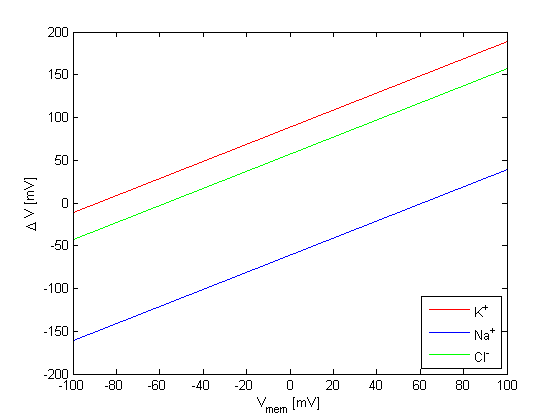
\includegraphics[scale=0.7]{../pics/drivingforce}
\caption{The driving force $\Delta \si{V}$ as a function of the membrane potential $\si{V}_{\text{mem}}$ for the potassium, sodium and chloride ions.}
\end{figure}

\section{Goldman equation}
\Question
\begin{enumerate}
\item
Assuming the concentrations you used for solving the Nernst equation, calculate the resting potential \textbf{for equal permeabilities} ($b=c=1$)!
\item
Calculate the resting potential for $b = 0.03$ and $c = 0.1$!
\end{enumerate}

\Answer\\
We insert the given values into the Goldman equation:
\begin{equation*}
E_{\text{rest}} = 27 \si{mV} \cdot \ln \frac{[\text{K}^+]_{\text{out}} + b [\text{Na}^+]_{\text{out}} + c [\text{Cl}^-]_{\text{in}}}{[\text{K}^+]_{\text{in}} + b [\text{Na}^+]_{\text{in}} + c [\text{Cl}^-]_{\text{out}}}
\end{equation*}

\begin{enumerate}
\item
\begin{equation*}
E_{\text{rest}} = 27 \si{mV} \cdot \ln \frac{5 \si{mM} + 145 \si{mM} + 13 \si{mM}}{140 \si{mM} + 15 \si{mM} + 110 \si{mM}}  \approx -13.12 \si{mV}
\end{equation*}
\item
\begin{equation*}
E_{\text{rest}} = 27 \si{mV} \cdot \ln \frac{5 \si{mM} + 0.03 \cdot 145 \si{mM} + 0.1 \cdot 13 \si{mM}}{140 \si{mM} + 0.03 \cdot 15 \si{mM} + 0.1 \cdot 110 \si{mM}} \approx -71.68 \si{mV}
\end{equation*}

\end{enumerate}


\end{document}














